\documentclass{standalone}
\usepackage{tikz}
\usetikzlibrary{positioning}

\begin{document}

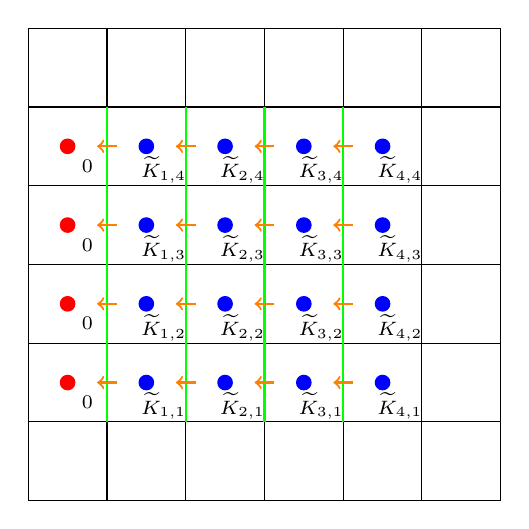
\begin{tikzpicture}
  % Draw the grid
  \foreach \x in {0,1,...,6} {
    \draw (\x,0) -- (\x,6);
  }
  \foreach \y in {0,1,...,6} {
    \draw (0,\y) -- (6,\y);
  }

  \foreach \x in {1,...,4} {
     \draw[green, thick] (\x,1) -- (\x,5); 
  }
  \foreach \x in {1, ..., 4}{
    \foreach \y in {1, ..., 4}{
      \draw[orange, thick, <-] (\x-0.125, \y+0.5) -- (\x+0.125, \y+0.5);
    }
  }

  % Add center points with color
  \foreach \i in {1,...,4} {
    \foreach \j in {1,...,4} {
        \node (a) at (\i+0.5, \j+0.5) [circle, fill=blue, inner sep=2pt] {};
        \node (b) at ([xshift=0.22cm, yshift=-0.3cm]a)  [font=\scriptsize]{$\widetilde{\boldmath{K}}_{\i,\j}$};
    }
  }
  % Left
  \foreach \i in {2, 3, 4, 5}{
    \node (a) at (0.5, \i-0.5) [circle, fill=red, inner sep=2pt] {};
    \node (b) at ([xshift=0.25cm, yshift=-0.25cm]a) [font=\scriptsize] {$0$};

  }


\end{tikzpicture}

\end{document}


      